\section{Evaluation}
\label{kvdirect:sec:eval}

\begin{figure}[t]
\subfloat[Fix memory utilization 0.5.\label{kvdirect:fig:optimize_fix_mem}]
{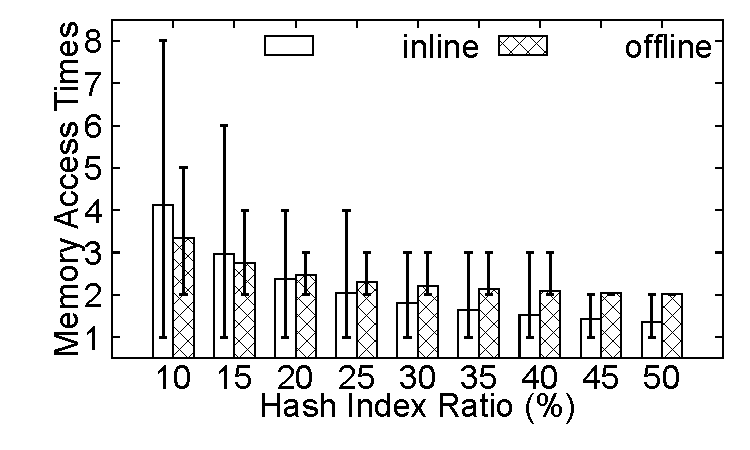
\includegraphics[width=.5\textwidth,page=1]{fix_mem.pdf}}
\subfloat[Fix hash index ratio 0.5.\label{kvdirect:fig:optimize_fix_ratio}]
{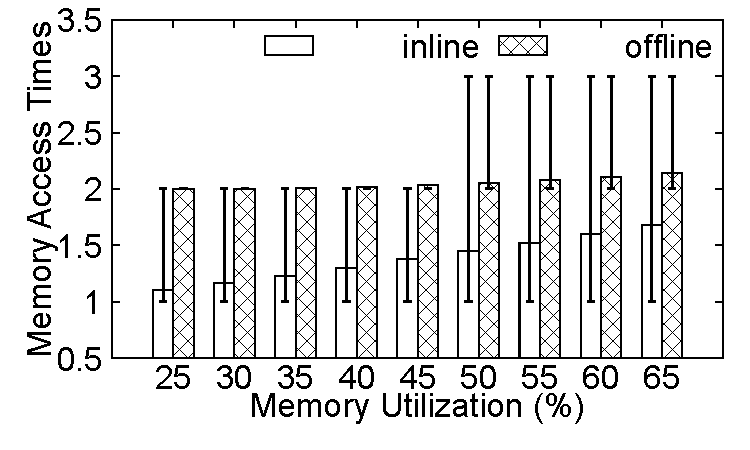
\includegraphics[width=.5\textwidth,page=1]{fix_ratio.pdf}}
\caption{Memory access count under different memory utilizations or hash index ratio.}
\label{kvdirect:fig:memory-access-count}
\end{figure}

\label{kvdirect:sec:evaluation}
In this section, we first take a reductionist perspective to support our design choices with microbenchmarks of key components, then switch to a holistic approach to demonstrate the overall performance of \oursys{} in system benchmark.

\label{kvdirect:sec:evaluation-setup}
We evaluate KV-Direct in a testbed of eight servers and one Arista DCS-7060CX-32S switch.
Each server equips two 8 core Xeon E5-2650 v2 CPUs with hyper-threading disabled, forming two NUMA nodes connected through QPI Link. Each NUMA node is populated with 8 DIMMs of 8~GiB Samsung DDR3-1333 ECC RAM, resulting a total of 128~GiB of host memory on each server.
A programmable NIC~\cite{caulfield2016cloud} is connected to the PCIe root complex of CPU 0, and its 40~Gbps Ethernet port is connected to the switch. The programmable NIC has two PCIe Gen3 x8 links in a bifurcated Gen3 x16 physical connector.
The tested server equips SuperMicro X9DRG-QF motherboard and one 120~GB SATA SSD running Archlinux (kernel 4.11.9-1).

For system benchmark, we use YCSB workload~\cite{cooper2010benchmarking}.
For skewed Zipf workload, we choose skewness 0.99 and refer it as \textit{long-tail} workload.

\subsection{Microbenchmarks}
\label{kvdirect:sec:microbenchmarks}


\begin{figure}[t]
\centering
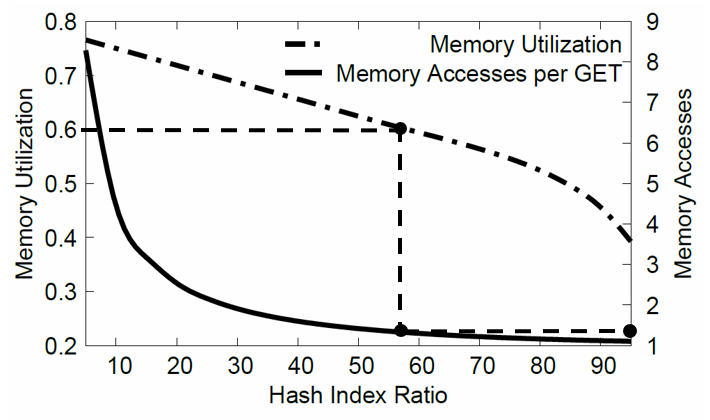
\includegraphics[width=0.6\textwidth,page=1]{optimize.png}
\caption{Determine the optimal hash index ratio for a required memory utilization and KV size.}
\label{kvdirect:fig:hashline-ratio}

\end{figure}

\subsubsection{Hash Table}
\label{kvdirect:sec:hashtable-eval}

There are two free parameters in our hash table design: (1) inline threshold, (2) the ratio of hash index in the entire memory space.
As shown in Figure~\ref{kvdirect:fig:optimize_fix_mem}, when hash index ratio grows, more KV pairs can be stored inline, yielding a lower average memory access time.
Figure~\ref{kvdirect:fig:optimize_fix_ratio} shows the increase of memory accesses as more memory is utilized.
As shown in Figure~\ref{kvdirect:fig:hashline-ratio}, the maximal achievable memory utilization drops under higher hash index ratio, because less memory is available for dynamic allocation.
Consequently, aiming to accommodate the entire corpus in a given memory size, the hash index ratio has an upper bound.
We choose this upper bound and get a minimal average memory access times, shown as the dashed line in Figure~\ref{kvdirect:fig:hashline-ratio}.

\begin{figure}[t]
\centering
\subfloat[10B GET.\label{kvdirect:fig:mem-access-10-get}]
{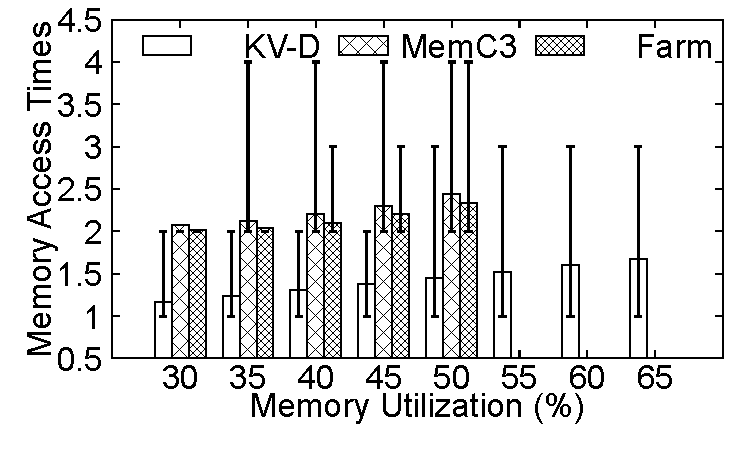
\includegraphics[width=.5\textwidth,page=1]{10B_get.pdf}}
\subfloat[10B PUT.\label{kvdirect:fig:mem-access-10-put}]
{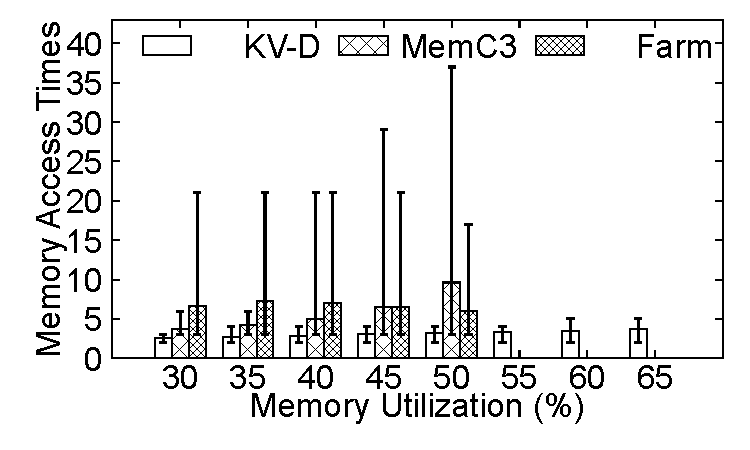
\includegraphics[width=.5\textwidth,page=1]{10B_put.pdf}}

\vfill

\subfloat[254B GET.\label{kvdirect:fig:mem-access-254-get}]
{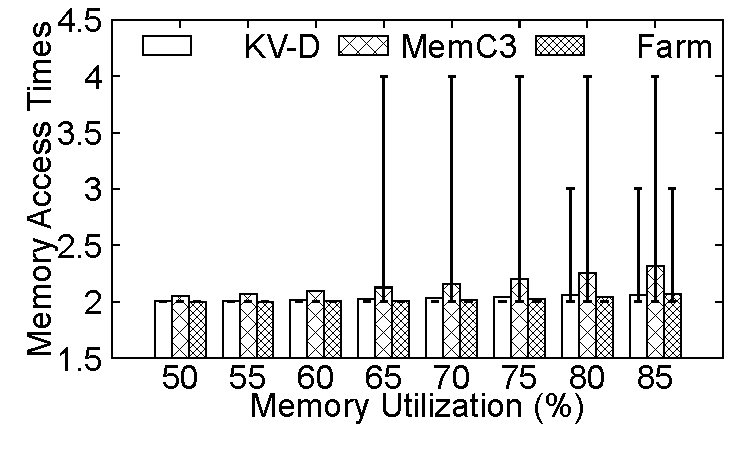
\includegraphics[width=.5\textwidth,page=1]{254B_get.pdf}}
\subfloat[254B PUT.\label{kvdirect:fig:mem-access-254-put}]
{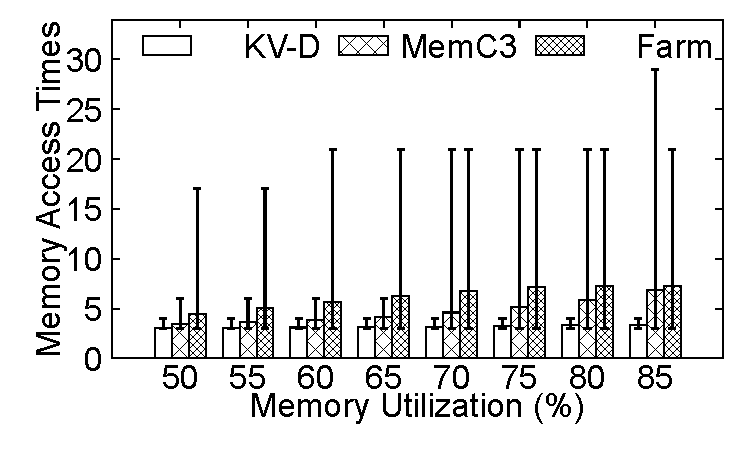
\includegraphics[width=.5\textwidth,page=1]{254B_put.pdf}}
\caption{Memory accesses per KV operation.}
\label{kvdirect:fig:mem-access-tput}

\end{figure}

In Figure~\ref{kvdirect:fig:mem-access-tput}, we plot the number of memory accesses per GET and PUT operation for three possible hash table designs: chaining in KV-Direct, bucket cuckoo hashing in MemC3~\cite{fan2013memc3} and chain-associative hopscotch hashing in FaRM~\cite{dragojevic2014farm}.
For KV-Direct, we make the optimal choice of inline threshold and hash index ratio for the given KV size and memory utilization requirement.
For cuckoo and hopscotch hashing, we assume that keys are inlined and can be compared in parallel, while the values are stored in dynamically allocated slabs.
Since the hash table of MemC3 and FaRM cannot support more than 55\% memory utilization for 10B KV size, the three rightmost bars in Figure~\ref{kvdirect:fig:mem-access-10-get} and Figure~\ref{kvdirect:fig:mem-access-10-put} only show the performance of KV-Direct.

For inline KVs, KV-Direct has close to 1 memory access per GET and close to 2 memory accesses per PUT under non-extreme memory utilizations.
GET and PUT for non-inline KVs have one additional memory access.
Comparing KV-Direct and chained hopscotch hashing under high memory utilization, hopscotch hashing performs better in GET, but significantly worse in PUT.
Although KV-Direct cannot guarantee worst case DMA accesses, we strike for a balance between GET and PUT.
Cuckoo hashing needs to access up to two hash slots on GET, therefore has more memory accesses than KV-Direct under most memory utilizations.
Under high memory utilization, cuckoo hashing incurs large fluctuations in memory access times per PUT.



\begin{figure}[t]
\centering
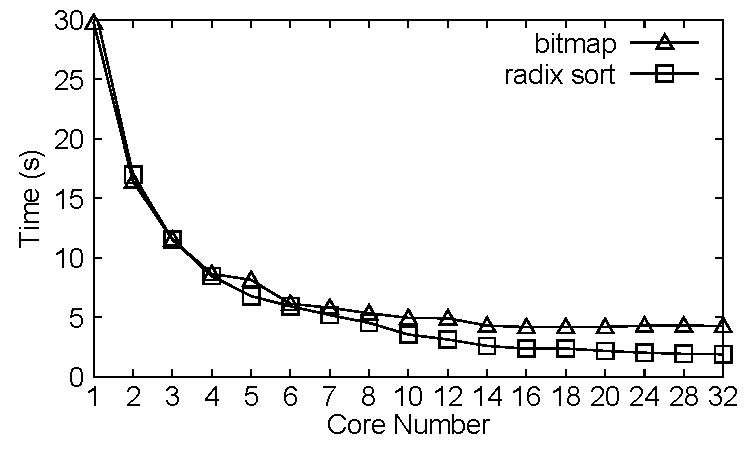
\includegraphics[width=0.6\textwidth]{slab-gc.pdf}
\caption{Execution time of merging 4 billion slab slots.}
\label{kvdirect:fig:slab-garbage-collection}

\end{figure}

\subsubsection{Slab Memory Allocator}
\label{kvdirect:sec:slab-eval}

The communication overhead of slab memory allocator comes from the NIC accessing available slab queues in host memory.
To sustain the maximal throughput of 180M operations per second, in the worst case, 180M slab slots need to be transferred, consuming 720 MB/s PCIe throughput, \ie, 5\% of total PCIe throughput of our NIC.

The computation overhead of slab memory allocator comes from slab splitting and merging on host CPU.
Fortunately, they are not frequently invoked.
For workloads with stable KV size distributions, newly freed slab slots are reused by subsequent allocations, therefore does not trigger splitting and merging.

Slab splitting requires moving continuous slab entries from one slab queue to another. When the workload shifts from large KV to small KV, in the worst case the CPU needs to move 90M slab entries per second, which only utilizes 10\% of a core because it is simply continuous memory copy.

Merging free slab slots to larger slots is rather a time-consuming task, because it involves filling the allocation bitmap with potentially random offsets and thus requiring random memory accesses.
To sort the addresses of free slabs and merge continuous ones, radix sort~\cite{satish2010fast} scales better to multiple cores than simple bitmap.
As shown in Figure~\ref{kvdirect:fig:slab-garbage-collection}, merging all 4 billion free slab slots in a 16 GiB vector requires 30 seconds on a single core, or only 1.8 seconds on 32 cores using radix sort~\cite{satish2010fast}.
Although garbage collecting free slab slots takes seconds, it runs in background without stalling the slab allocator, and practically only triggered when the workload shifts from small KV to large KV.

\begin{figure}[t]
\centering
\subfloat[Atomics.\label{kvdirect:fig:ooo-atomic}]
{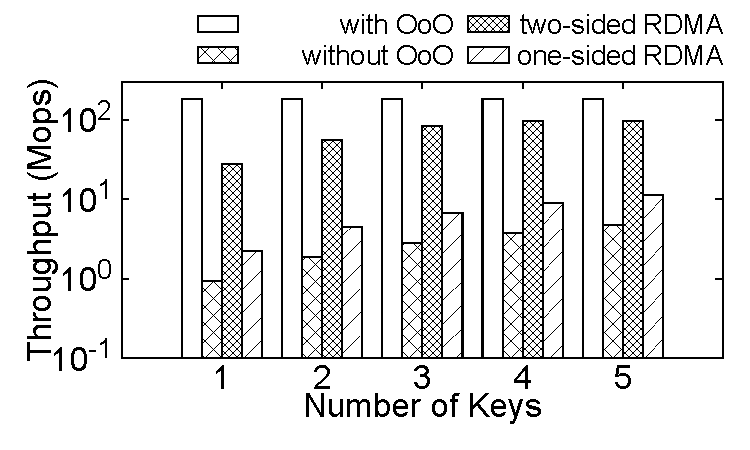
\includegraphics[width=.5\textwidth,page=1]{ooo_atomic.pdf}}
\subfloat[Long-tail workload.\label{kvdirect:fig:ooo-longtail}]
{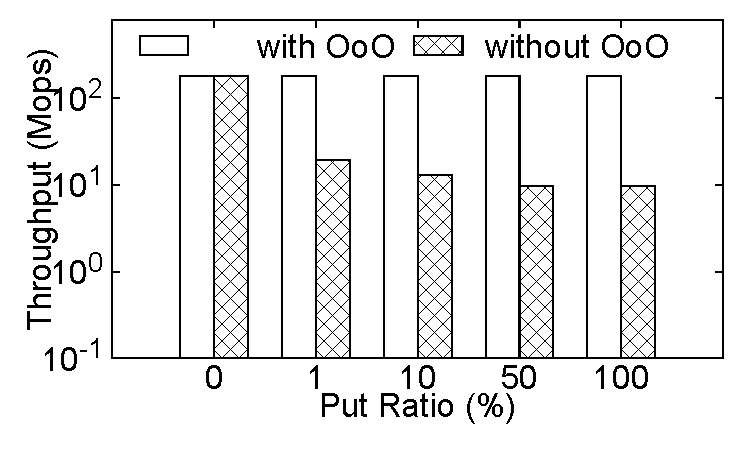
\includegraphics[width=.5\textwidth,page=1]{ooo_long-tail.pdf}}
\caption{Effectiveness of out-of-order execution engine.}
\label{kvdirect:fig:ooo-eval}

\end{figure}


\subsubsection{Out-of-Order Execution Engine}
\label{kvdirect:sec:ooo-eval}

We evaluate the effectiveness of out-of-order execution by comparing the throughput with the simple approach that stalls the pipeline on key conflict, under atomics and long-tail workload. One-sided RDMA and two-sided RDMA~\cite{kalia2016design} throughputs are also shown as baselines.

Without this engine, an atomic operation needs to wait for PCIe latency and processing delay in the NIC, during which subsequent atomic operations on the same key cannot be executed.
This renders a single-key atomics throughput of 0.94~Mops in Figure~\ref{kvdirect:fig:ooo-atomic}, consistent with 2.24~Mops measured from an RDMA NIC~\cite{kalia2016design}.
The higher throughput of RDMA NIC can be attributed to its higher clock frequency and lower processing delay.
With out-of-order execution, single-key atomic operations in KV-Direct can be processed at peak throughput, \ie, one operation per clock cycle.
In MICA~\cite{lim2014mica}, single-key atomics throughput cannot scale beyond a single core.
Atomic fetch-and-add can be spread to multiple cores in~\cite{kalia2016design}, but it relies on the commutativity among the atomics and therefore does not apply to non-commutative atomics such as compare-and-swap.

With out-of-order execution, single-key atomics throughput improves by 191x and reaches the clock frequency bound of 180~Mops.
When the atomic operations spread uniformly among multiple keys, the throughput of one-sided RDMA, two-sided RDMA and KV-Direct without out-of-order execution grow linearly with the number of keys, but still far from the optimal throughput of KV-Direct.

Figure~\ref{kvdirect:fig:ooo-longtail} shows the throughput under the long-tail workload.
Recall that the pipeline is stalled when a PUT operation finds any in-flight operation with the same key.
The long-tail workload has multiple extremely popular keys, so it is likely that two operations with the same popular key arrive closely in time.
With higher PUT ratio, it is more likely that at least one of the two operations is a PUT, therefore triggering a pipeline stall.


\begin{figure}[t]
\centering
{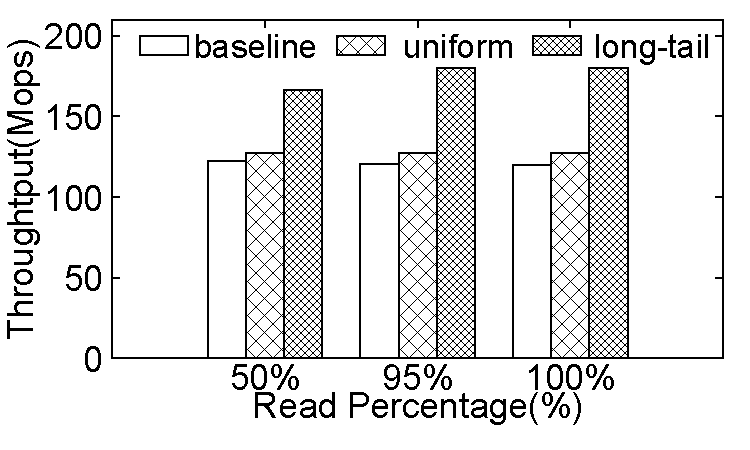
\includegraphics[width=.5\textwidth,page=1]{load_balancer.pdf}}
\caption{DMA throughput with load dispatch (load dispatch ratio = 0.5).}
\label{kvdirect:fig:cache-tput}

\end{figure}

\subsubsection{DRAM Load Dispatcher}
\label{kvdirect:sec:dram-eval}

Figure~\ref{kvdirect:fig:cache-tput} shows the throughput improvement of DRAM load dispatch over the baseline of using PCIe only.
Under uniform workload, the caching effect of DRAM is negligible because its size is only 6\% of host KVS memory.
Under long-tail workload, \approx30\% of memory accesses are served by the DRAM cache. Overall, the memory access throughput for 95\% and 100\% GET achieves the 180 Mops clock frequency bound.
However, if DRAM is simply used as a cache, the throughput would be adversely impacted because the DRAM throughput is lower than PCIe throughput.

\subsubsection{Vector Operation Decoder}
\label{kvdirect:network-eval}

\begin{table}[]
\centering
\scalebox{0.8}{
\begin{tabular}{|l|r|r|r|r|r|}
\hline
Vector Size (B)              & 64    & 128   & 256   & 512   & 1024  \\ \hline
Vector update with return    & 11.52 & 11.52 & 11.52 & 11.52 & 11.52 \\ \hline
Vector update without return & 4.37  & 4.53  & 4.62  & 4.66  & 4.68  \\ \hline
One key per element          & 2.09  & 2.09  & 2.09  & 2.09  & 2.09  \\ \hline
Fetch to client              & 0.03  & 0.06  & 0.12  & 0.24  & 0.46  \\ \hline
\end{tabular}
}
\caption{Throughput (GB/s) of vector operations with vector update or alternatives.}
\label{kvdirect:tab:vec_throughput}

\end{table}

To evaluate the efficiency of vector operations in KV-Direct,
Table~\ref{kvdirect:tab:vec_throughput} compares the throughput of atomic vector increment with two alternative approaches:
(1) If each element is stored as a unique key, the bottleneck is the network to transfer the KV operations.
(2) If the vector is stored as a large opaque value, retrieving the vector to the client also overwhelms the network.
Additionally, the two alternatives in Table~\ref{kvdirect:tab:vec_throughput} do not ensure consistency within the vector. Adding synchronization would incur further overhead.


\begin{figure}[t]
\centering
\subfloat[Throughput.\label{kvdirect:fig:network-batching-bw}]
{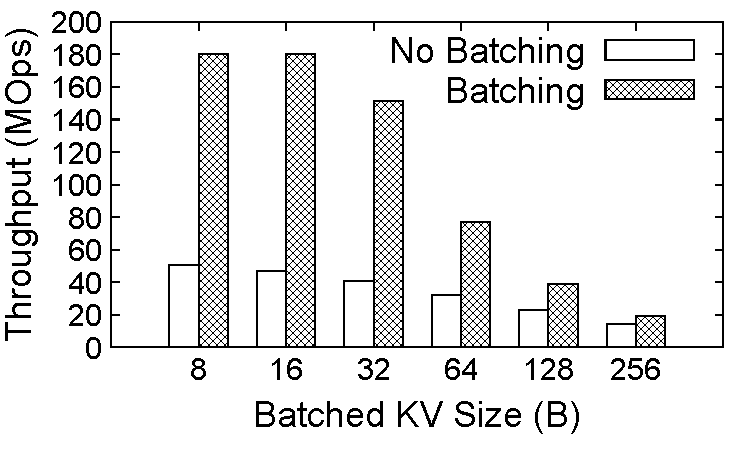
\includegraphics[width=.5\textwidth,page=1]{net_batching_bw.pdf}}
\subfloat[Latency.\label{kvdirect:fig:network-batching-bw}]
{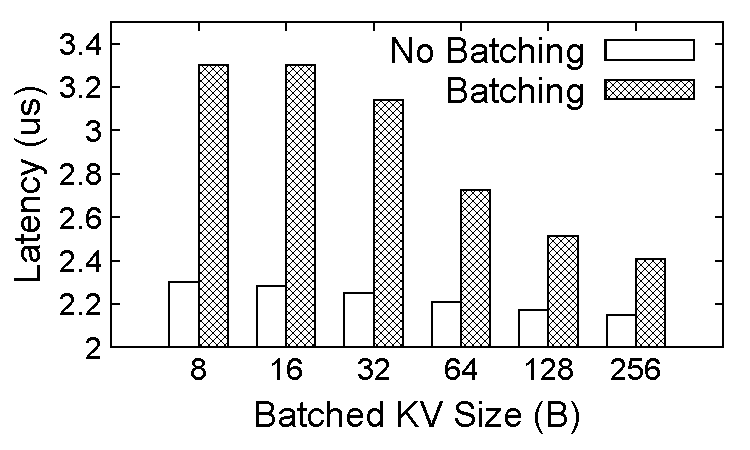
\includegraphics[width=.5\textwidth,page=1]{net_batching_lat.pdf}}
\caption{Efficiency of network batching.}
\label{kvdirect:fig:eval-network-batching}

\end{figure}

KV-Direct client packs KV operations in network packets to mitigate packet header overhead.
Figure~\ref{kvdirect:fig:eval-network-batching} shows that network batching increases network throughput by up to 4x, while keeping networking latency below 3.5~$\mu$s.

\egg{
\subsubsection{Congestion Avoidance}
\label{kvdirect:congestion-avoidance}

We evaluate the efficiency of congestion avoidance using the KV size distribution of the USR pool in Facebook memcached workload~\cite{atikoglu2012workload}.
As shown in Figure~\ref{kvdirect:fig:congestion-avoidance}, without congestion avoidance, about 70\% KV operations complete with close to one PCIe RTT latency, while remaining 30\% operations have inflated completion times due to explicit and implicit queuing in the KV processor.
With congestion avoidance, the rate for the programmable NIC to accept KV operations from clients is dynamically adjusted, therefore $>$~90\% KV operations complete with close to one PCIe RTT latency.
The remaining few percent of operations have intrinsic higher processing delay due to their larger KV sizes.
}

\subsection{System Benchmark}
\label{kvdirect:sec:system-benchmark}

\subsubsection{Methodology}

Before each benchmark, we tune hash index ratio, inline threshold and load dispatch ratio according to the KV size, access pattern and target memory utilization.
Then we generate random KV pairs with a given size.
The key size in a given inline KV size is irrelevant to the performance of KV-Direct, because the key is padded to the longest possible inline KV size during processing.
To test inline case, we use KV size that is a multiple of slot size (when size $\leq$ 50, \textit{i.e.} 10 slots). To test non-inline case, we use KV size that is a power of two minus 2 bytes (for metadata).
As the last step of preparation, we issue PUT operations to insert the KV pairs into an idle KVS until 50\% memory utilization.
The performance under other memory utilizations can be derived from Figure~\ref{kvdirect:fig:mem-access-tput}.

During benchmark, we use an FPGA-based packet generator~\cite{li2016clicknp} in the same ToR to generate batched KV operations, send them to the KV server, receive completions and measure sustainable throughput and latency.
The processing delay of the packet generator is pre-calibrated via direct loop-back and removed from latency measurements.
Error bars represent the $5^{th}$ and $95^{th}$ percentile.

\subsubsection{Throughput}

\begin{sidewaystable}[h]
\centering
\begin{tabular}{|l|l|l|r|r|r|r|r|r|r|}
\toprule
KVS  & Comment & Bottleneck & \multicolumn{2}{c|}{Tput (Mops)} & \multicolumn{2}{c|}{Power Efficiency (Kops/W)} & \multicolumn{2}{c|}{Avg Delay ($\mu$s)} \\
\cline{4-9}
 & & & GET & PUT & GET & PUT & GET & PUT \\
\midrule
Memcached~\cite{fitzpatrick2004distributed} & Traditional & Core synchronization & 1.5 & 1.5 & \approx5 & \approx5 & \approx50 & \approx50 \\
MemC3~\cite{fan2013memc3} & Traditional & OS network stack & 4.3 & 4.3 & \approx14 & \approx14 & \approx50 & \approx50 \\
RAMCloud~\cite{ousterhout2015ramcloud} & Kernel bypass & Dispatch thread & 6 & 1 & \approx20 & \approx3.3 & 5 & 14 \\
MICA~\cite{lim2014mica} & Kernel bypass, 24 cores, 12 NIC ports & CPU KV processing & 137 & 135 & 342 & 337 & 81 & 81 \\
FaRM~\cite{dragojevic2014farm} & One-sided RDMA for GET & RDMA NIC & 6 & 3 & \approx30 (261) & \approx15 & 4.5 & \approx10 \\
DrTM-KV~\cite{wei2015fast} & One-sided RDMA and HTM & RDMA NIC & 115.2 & 14.3 & \approx500 (3972) & \approx60 & 3.4 & 6.3 \\
HERD'16~\cite{kalia2016design} & Two-sided RDMA, 12 cores & PCIe & 98.3 & \approx60 & \approx490 & \approx300 & 5 & 5 \\
Xilinx'13~\cite{blott13hotcloud} & FPGA (with host) & Network & 13 & 13 & 106 & 106 & 3.5 & 4.5 \\
Mega-KV~\cite{zhang2015mega} & GPU (4~GiB on-board RAM) & GPU KV processing & 166 & 80 & \approx330 & \approx160 & 280 & 280 \\
\midrule
\textbf{KV-Direct (1 NIC)} & Programmable NIC, two Gen3 x8 & PCIe \& DRAM & 180 & 114 & 1487 (5454) & 942 (3454) & 4.3 & 5.4 \\
\textbf{KV-Direct (10 NICs)} & Programmable NIC, one Gen3 x8 each & PCIe \& DRAM & 1220 & 610 & 3417 (4518) & 1708 (2259) & 4.3 & 5.4 \\
\bottomrule
\end{tabular}
\caption{Comparison of KV-Direct with other KVS systems under long-tail (skewed Zipf) workload of 10B tiny KVs. For metrics not reported in the papers, we emulate the systems using similar hardware and report our approximate measurements. For CPU-bypass systems, numbers in parentheses report power difference under peak load and idle.}
\label{kvdirect:tab:kvs-compare}

\end{sidewaystable}

\begin{figure}[t]
\centering
\subfloat[Uniform.\label{kvdirect:fig:ycsb-tput-uniform}]
{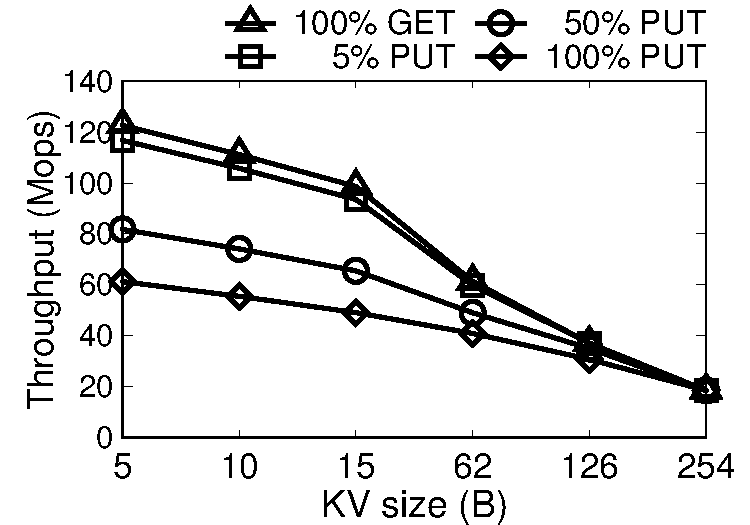
\includegraphics[width=.5\textwidth,page=1]{ycsb-tput-uniform.pdf}}
\subfloat[Long-tail.\label{kvdirect:fig:ycsb-tput-longtail}]
{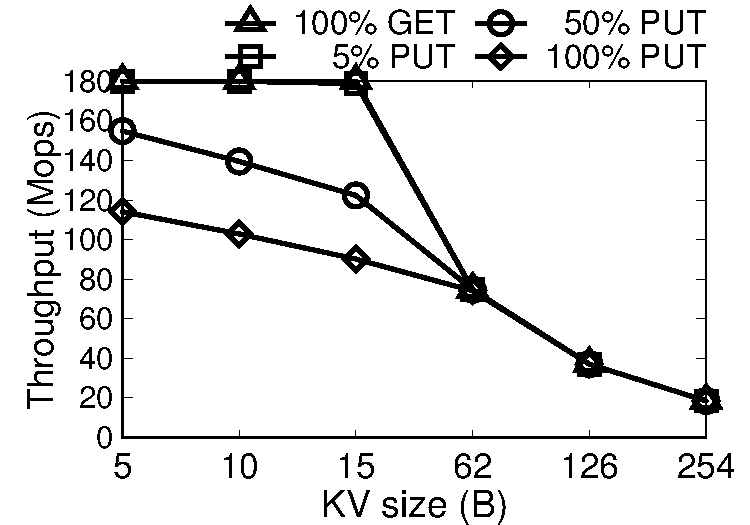
\includegraphics[width=.5\textwidth,page=1]{ycsb-tput-longtail.pdf}}
\caption{Throughput of KV-Direct under YCSB workload.}
\label{kvdirect:fig:ycsb-tput}

\end{figure}

Figure~\ref{kvdirect:fig:ycsb-tput} shows the throughput of KV-Direct under YCSB uniform and long-tail (skewed Zipf) workload.
Three factors may be the bottleneck of KV-Direct: clock frequency, network and PCIe/DRAM.
For 5B\approx15B KVs inlined in the hash index, most GETs require one PCIe/DRAM access and PUTs require two PCIe/DRAM accesses.
Such tiny KVs are prevalent in many systems. In PageRank, the KV size for an edge is 8B. In sparse logistic regression, the KV size is typically 8B-16B. For sequencers and locks in distributed systems, the KV size is 8B.

Under same memory utilization, larger inline KVs have lower throughput, due to a higher probability of hash collision.
62B and larger KVs are not inlined, so they require an additional memory access.
Long-tail workload has higher throughput than uniform workload and able to reach the clock frequency bound of 180~Mops under read-intensive workload, or reach the network throughput bound for $\geq$62B KV sizes.
Under long-tail workload, the out-of-order execution engine merges up to \approx15\% operations on the most popular keys, and the on-board DRAM has \approx60\% cache hit rate under 60\% load dispatch ratio, which collectively lead to up to 2x throughput as uniform workload.
As shown in Table~\ref{kvdirect:tab:kvs-compare}, the throughput of a KV-Direct NIC is on-par with a state-of-the-art KVS server with tens of CPU cores.

\subsubsection{Power efficiency}

%Plugging a KV-Direct NIC adds 10.6~W power to the idle server.
When the KV-Direct server is at peak throughput, the system power is 121.4 watts (measured on the wall).
Compared with state-of-the-art KVS systems in Table~\ref{kvdirect:tab:kvs-compare}, KV-Direct is 3x more power efficient than other systems, being the first general-purpose KVS system to achieve 1 million KV operations per watt on commodity servers.

When the KV-Direct NIC is unplugged, an idle server consumes 87.0 watts power, therefore the combined power consumption of programmable NIC, PCIe, host memory and the daemon process on CPU is only 34 watts.
Measured power difference is justified since the CPU is almost idle and the server can run other workloads when KV-Direct is operating (we use the same criterion for one-sided RDMA, shown at parentheses of Table~\ref{kvdirect:tab:kvs-compare}).
In this regard, KV-Direct is 10x more power efficient than CPU-based systems.

\subsubsection{Latency}
\begin{figure}[t]
\centering
\subfloat[With batching.\label{kvdirect:fig:ycsb-lat-batch}]
{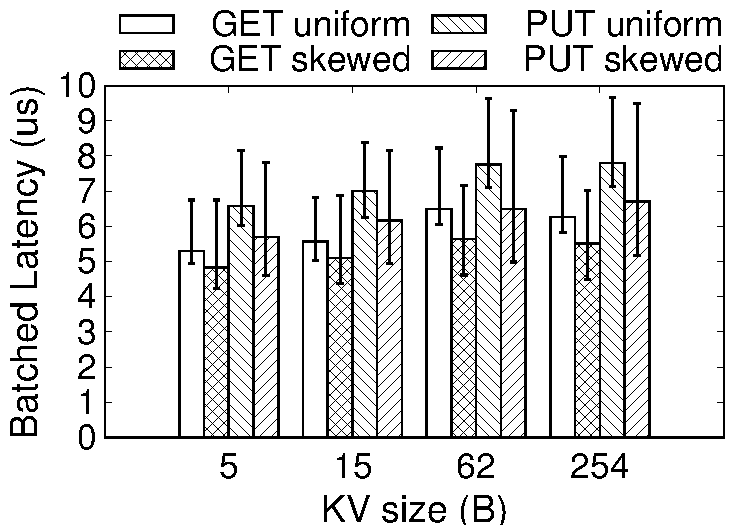
\includegraphics[width=.5\textwidth,page=1]{lat-batch.pdf}}
\subfloat[Without batching.\label{kvdirect:fig:ycsb-lat-nobatch}]
{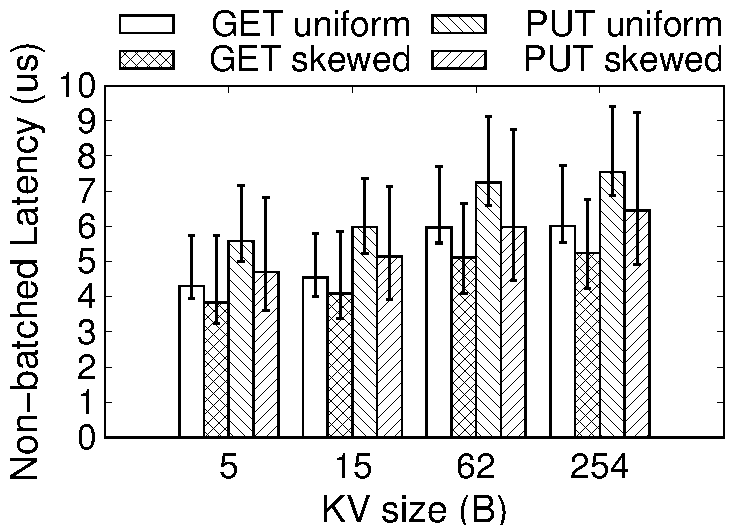
\includegraphics[width=.5\textwidth,page=1]{lat-nonbatch.pdf}}
\caption{Latency of KV-Direct under peak throughput of YCSB workload.}
\label{kvdirect:fig:ycsb-lat}

\end{figure}

Figure~\ref{kvdirect:fig:ycsb-lat} shows the latency of KV-Direct under the peak throughput of YCSB workload.
Without network batching, the tail latency ranges from 3\approx9~$\mu$s depending on KV size, operation type and key distribution.
PUT has higher latency than GET due to additional memory access.
Skewed workload has lower latency than uniform due to more likelihood of being cached in on-board DRAM.
Larger KV has higher latency due to additional network and PCIe transmission delay.
Network batching adds less than 1~$\mu$s latency than non-batched operations, but significantly improves throughput, which has been evaluated in Figure~\ref{kvdirect:fig:eval-network-batching}.

\subsubsection{Impact on CPU performance}

\begin{table}[t!]
	\centering
		\begin{tabular}{l|l|r|r}
			\toprule
			\multicolumn{2}{r}{KV-Direct status $\rightarrow$} & Idle & Busy \\
			\midrule
			\multirow{4}{*}{\specialcell{Random\\Latency}} & CPU0-0 & 82.2 ns & 83.5 ns \\
            					  & CPU0-1 & 129.3 ns & 129.9 ns \\
                                  & CPU1-0 & 122.3 ns & 122.2 ns \\
                                  & CPU1-1 & 84.2 ns & 84.3 ns \\
			\midrule
            \multirow{4}{*}{\specialcell{Sequential\\Throughput}} & \textbf{CPU0-0} & \textbf{60.3 GB/s} & \textbf{55.8 GB/s} \\
            					  & CPU0-1 & 25.7 GB/s & 25.6 GB/s \\
                                  & CPU1-0 & 25.5 GB/s & 25.9 GB/s \\
                                  & CPU1-1 & 60.2 GB/s & 60.3 GB/s \\
			\midrule
			\multirow{4}{*}{\specialcell{Random\\Throughput}} & 32B read & 10.53 GB/s & 10.46 GB/s \\
            						& 64B read & 14.41 GB/s & 14.42 GB/s \\
                                    & 32B write & 9.01 GB/s & 9.04 GB/s \\
                                    & 64B write & 12.96 GB/s & 12.94 GB/s \\
			\bottomrule
		\end{tabular}
    	\caption{Impact on CPU memory access performance when KV-Direct is at peak throughput. Measured with Intel Performance Counter Monitor V2.11.}
        \label{kvdirect:tab:cpu-impact}
        
\end{table}


KV-Direct is designed to bypass the server CPU and uses only a portion of host memory for KV storage. Therefore, the CPU can still run other applications.
Our measurements find a minimal impact on other workloads on the server when a single NIC KV-Direct is at peak load.
Table~\ref{kvdirect:tab:cpu-impact} quantifies this impact at the peak throughput of KV-Direct.
Except for sequential throughput of CPU 0 to access its own NUMA memory (the line marked in bold), the latency and throughput of CPU memory accesses are mostly unaffected.
This is because 8 channels of host memory can provide far higher random access throughput than all CPU cores could consume, while the CPU can indeed stress the sequential throughput of the DRAM channels.
The impact of the host daemon process is minimal when the distribution of KV sizes is relatively stable, because the garbage collector is invoked only when the number of available slots for different slab sizes are imbalanced.
